% ---
% Capitulo de Desenvolvimento da Aplicação
% ---
\chapter{Desenvolvimento}
% ---
Este capítulo apresenta o projeto do \textit{Business Intelligence} do Setor de Nutrição Clínica do HU-UFS abordando estratégias, necessidades informacionais e peculiaridades do setor de nutrição do hospital. Serão descritas as atividades de criação do modelo relacional do \textit{Datawarehouse}, detalhamento do processo de ETL e a elaboração da interface OLAP. São apresentados também a interface web destinada aos tomadores de decisão, os resultados das consultas OLAP e informações referentes ao escopo do projeto e ao HU-UFS.
% ---
\section{Hospital Universitário de Aracaju - HU-UFS}
% ---
O Hospital Universitário (HU) é um campus da Universidade Federal de Sergipe (UFS) desde 1984, funcionando como centro hospitalar de assistência, ensino e pesquisa em ciências da saúde. Atualmente, o HU-UFS em Sergipe ocupa um espaço de referência e excelência na prestação de assistência médico-hospitalar de média e alta complexidade \cite{sitehuufs}.

Em 2013, a UFS e a Empresa Brasileira de Serviços Hospitalares (EBSERH) firmaram convênio para transferência da administração do HU no âmbito do Programa Nacional de Reestruturação dos Hospitais Universitários Federais (REHUF). O HU-UFS tornou-se a nona filial da EBSERH com administração vigorosa em todas as áreas do hospital. Em abril de 2016, o HU-UFS tornou-se habilitado para o atendimento especializado de pessoas com deficiência auditiva, bem como para procedimentos de vasectomia. Atualmente, a estrutura do hospital inclui departamentos de Clínica Médica, Clínica Cirúrgica, Pediatria, Unidade de Terapia Intensiva (UTI) e Centro Cirúrgico. Vários cursos de graduação, pós-graduação, residência médica e multiprofissional utilizam as instalações desse hospital-escola para desenvolver práticas e pesquisas inovadoras \cite{sitehuufs}. 

% ---
\section{Escopo do Projeto}
% ---
A Unidade de Nutrição Clínica do HU armazena seus registros de formulários de acompanhamento nutricional dos pacientes em planilhas eletrônicas. As informações entregues à gestão do hospital são consultadas nestas planilhas pela chefia do setor. Os dados mais relevantes para a chefia estão relacionadas aos índices de classificação de risco, estado nutricional, utilização de suplementação e utilização de dietas enterais e suas relações com possíveis complicações identificadas nos pacientes internados nas diversas clínicas do hospital. Um dos formulários utilizados para coleta de dados básicos para essas planilhas é apresentado na \autoref{fig_figuraFormularioDiagClinicoNutri}.

\begin{figure}[htb]
	\caption{\label{fig_figuraFormularioDiagClinicoNutri}Formulário de Diagnóstico Clínico-Nutricional.}
	\begin{center}
	    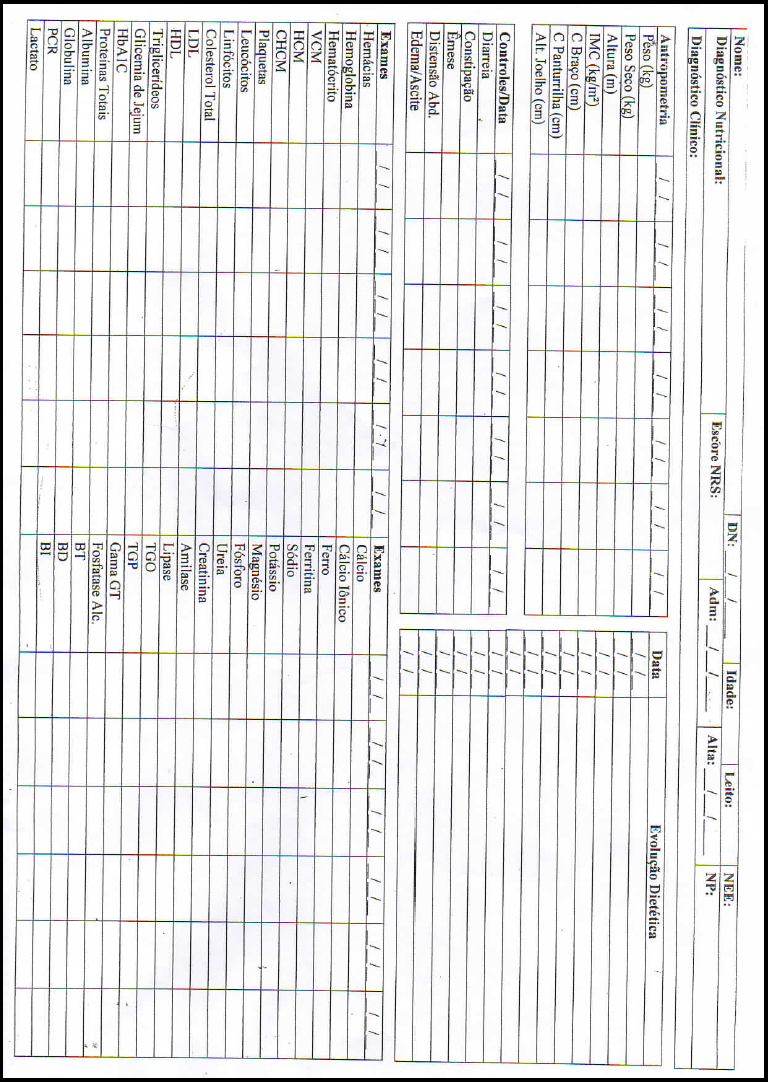
\includegraphics[scale=0.569]{Imagens/figura - formulario diagnostico clinico nutricional.png}
	\end{center}
	\legend{Fonte: \cite{huufs}.}
\end{figure}

Todos esses dados, antes de serem carregados no \textit{Data Warehouse} (DW) devem passar por um processo de ETL, que de forma sistemática realiza tratamento e limpeza dos dados advindos dos diversos arquivos fornecidos pela unidade de nutrição e pelo hospital. 

Um ponto importante a ser considerado, é que devido ao surto mundial de Sars-Cov-2, confirmado pela \citeonline{whocovid} em 2020, vários hospitais tiveram de passar por revisões dos seus protocolos de atendimento. Com a emissão de resolução do Conselho Federal de Nutrição e do Protocolo Operacional Padrão emitido pelo HU-UFS, a Unidade de Nutrição não mais realizou triagens nutricionais em pacientes de forma presencial e o acompanhamento nutricional foi realizado apenas de forma online e com regras diferentes para avaliação \cite{protocolocovidnutri, cfnutri646}. Com todas as mudanças ocorridas em 2020, a unidade não foi capaz de realizar o registro de alguns dados conforme padrão de anos anteriores e disponibilizou apenas a fonte de dados do ano de 2019 para consideração neste trabalho.

Com os dados disponíveis carregados no DW se faz necessário criar um modelo de dados OLAP, no qual as informações são organizadas conceitualmente em cubos de dados para análise dinâmica e multidimensional dos dados consolidados.

Com a possibilidade de consultas dinâmicas oferecidas pelo OLAP a Unidade de Nutrição Clínica solicitou além dos dados quantitativos também gráficos de comparação, composição e tendência para diferentes dimensões, sempre considerando uma visão de todo o hospital e uma visão por enfermaria como descritos abaixo: 

Para o indicador de Triagem Nutricional Realizada, as seguintes informações foram solicitados:
\begin{itemize}
    \item Quantidade de Triagens Nutricionais Realizadas ao Ano;
    \item Quantidade de Triagens Nutricionais Realizadas por Mês;
    \item Quantidade de Triagens Nutricionais Realizadas por Enfermaria ao Ano;
    \item Tendência de Triagens Nutricionais Realizadas por Enfermaria.
\end{itemize}

Para o indicador de Classificação de Risco foram solicitadas as seguintes informações:
\begin{itemize}
    \item Percentual de Triagem Nutricional por Classificação de Risco ao Ano;
    \item Percentual de Triagem Nutricional por Classificação de Risco detalhado por mês;
    \item Percentual de Triagem Nutricional por Classificação de Risco por Enfermaria ao Ano;
    \item Tendência de Triagem Nutricional por Classificação de Risco por Enfermaria detalhado por mês.
\end{itemize}

Para o indicador de Estado Nutricional foram solicitadas as seguintes informações:
\begin{itemize}
    \item Percentual de Triagem Nutricional por Estado Nutricional ao Ano;
    \item Percentual de Triagem Nutricional por Estado Nutricional detalhado por mês;
    \item Percentual de Triagem Nutricional por Estado Nutricional por Enfermaria ao Ano;
    \item Tendência de Triagem Nutricional por Estado Nutricional por Enfermaria detalhado por mês.
\end{itemize}

Para o indicador de Uso de Suplementação foram solicitadas as seguintes informações:
\begin{itemize}
    \item Percentual de Triagem Nutricional por Uso de Suplementação ao Ano;
    \item Percentual de Triagem Nutricional por Uso de Suplementação detalhado por mês;
    \item Percentual de Triagem Nutricional por Uso de Suplementação por Enfermaria ao Ano;
    \item Tendência de Triagem Nutricional por Uso de Suplementação por Enfermaria detalhado por mês.
    \item Quantidade de Pacientes em Uso de Suplemento
\end{itemize}

Para o indicador de Uso de Dieta Enteral foram solicitadas as seguintes informações:
\begin{itemize}
    \item Percentual de Triagem Nutricional por Uso de Dieta Enteral ao Ano;
    \item Percentual de Triagem Nutricional por Uso de Dieta Enteral detalhado por mês;
    \item Percentual de Triagem Nutricional por Uso de Dieta Enteral por Enfermaria ao Ano;
    \item Tendência de Triagem Nutricional por Uso de Dieta Enteral por Enfermaria detalhado por mês.
\end{itemize}

% ---
% primeiro capitulo de Resultados
% ---
\chapter{Considerações Finais}
% ---

% ---
\section{Vestibulum ante ipsum primis in faucibus orci luctus et ultrices
posuere cubilia Curae}
% ---

\lipsum[21-22]

% ---
% segundo capitulo de Resultados
% ---
\chapter{Nam sed tellus sit amet lectus urna ullamcorper tristique interdum
elementum}
% ---

% ---
\section{Pellentesque sit amet pede ac sem eleifend consectetuer}
% ---

\lipsum[24]